\chapter{MoSeL}
\label{chap:reimplementation_ipm}

The original implementation of Iris Proof Mode is due to \citet{krebbersInteractiveProofsHigherorder2017} and, as follows from the name, is a set of tactics to do interactive proofs in Coq in Iris.
It was later extended to MoSeL by \citet{krebbersMoSeLGeneralExtensible2018}, which is a general framework for modal separation logics in Coq.
The idea behind the proof mode is to provide users with separation-logic version of familiar Coq tactics, like \coqe{intros} or \coqe{destruct}.

In this chapter we describe the implementation of MoSeL as it is currently, with Ltac.
First we cover the basics of separation logic and its semantics, then describe the embedding of logic in Coq and what MoSeL entailments correspond to in Bunched Implications (BI) logic.
Finally, we go into the details of the implementation of tactics.

Please note, that, following the MoSeL paper \cite[Section 2]{krebbersMoSeLGeneralExtensible2018}, we focus on the BI -- the assertion language of separation logic, and not on Hoare triples.

\section{Introduction to separation logic}
\label{sec:separation-logic-intro}

We will now describe the basics of separation logic.
Separation logic is an extension of Hoare logic which includes several new operators, the most important two being separating conjunction \((*)\) and separating implication or ``magic wand'' \((\wand)\).
Separation logic is also built on Bunched Implications logic.

A BI logic is a set of propositions \Prop with an entailment predicate \(\vdash\) and the following connectives:
\begin{enumerate}
\item embedding of ``pure'' propositions from meta-logic, which don't concern resources: \(\pure { } : \textbf{Prop} \to \Prop\)
\item \True, a neutral element for non-separating conjunction \(\wedge : \Prop \to \Prop \to \Prop\)
\item \False, a neutral element for non-separating disjunction \(\vee : \Prop \to \Prop \to \Prop\)
\item \emp, a neutral element for separating conjunction \(* : \Prop \to \Prop \to \Prop\)
\item \(\imp\) and \(\wand\), two implication-like connectives, where only the latter is separating \(\wand, \imp : \Prop \to \Prop \to \Prop\).
\item quantifiers, since the logic is higher-order: \(\forall, \exists : \forall A, (A \to \Prop) \to \Prop\)
\end{enumerate}

Apart from the laws concerning neutral elements mentioned above, there are laws concerning introduction and elimination of connectives, as well as the usual properties like commutativity and associativity.

The connectives that differentiate BI logic from regular logic are separating conjunction (\(*\)) and magic wand (\(\wand\)).
Intuition behind BI logic is somewhat simpler to understand by example.
In classical separation logic \cite{reynoldsSeparationLogicLogic2002, ohearnLocalReasoningPrograms2001}, a prototypical instance of a BI logic, propositions are predicates on memory heaps.
In this case separating conjunction \(P \ast Q\) represents a proposition that asserts that the heap can be divided in two heaplets, such that they don't share any memory and that one satisfies \(P\), while the other satisfies \(Q\).
Separating implication \(P \wand Q\) asserts ownership of a heaplet, such that for any separate heaplet that satisfies \(P\), the two together satisfy \(Q\).
Lastly, the neutral element \emp simply means that the heap is empty.
Non-separating conjunction \(P \wedge Q \)in that case means that the heap satisfies both \(P\) and \(Q\) simultaneously.

The entailment predicate for BI takes a ``bunch'' for the context and a BI proposition for the goal.
Bunches can be formed by two connectives -- ``additive'', which is represented as a semincolon, and ``multiplicative'', which is represented by a comma.
The bunches are introduced by the following two introduction rules:
\begin{equation*}
  \infer[\textsc{Imp-Intro}]
        {\Gamma \vdash P \imp Q}
        {\Gamma ; P \vdash Q}
  \quad \quad \quad
  \infer[\textsc{Wand-Intro}]
        {\Gamma \vdash P \wand Q}
        {\Gamma , P \vdash Q}
\end{equation*}
Intuitively, the additive bunch corresponds to non-separating conjunction, while the multiplicative bunch to separating one.
\begin{equation*}
  \infer{P \wedge Q \vdash R}
        {P ; Q \vdash R}
  \quad \quad \quad \quad \quad
  \infer{P \ast Q \vdash R}
        {P, Q \vdash R}
\end{equation*}
The important distinction, however, is that additive bunches admit the rules of Weakening and Contraction, while in classical BI multiplicative bunches do not.
This is also reflected by the introduction rules for conjunctions:
\begin{equation*}
  \infer[\textsc{And-Intro}]
        {\Gamma \vdash P \wedge Q}
        {\Gamma \vdash P &
         \Gamma \vdash Q }
  \quad \quad \quad
  \infer[\textsc{Sep-Intro}]
        {\Gamma, \Delta \vdash P \ast Q}
        {\Gamma \vdash P &
         \Delta \vdash Q }
\end{equation*}

For more careful treatment of BI logic the reader is referred to the original works \cite{ohearnLogicBunchedImplications1999, pymSemanticsProofTheory2002a}.
We are, however, more interested in the separation logic that uses BI logic to describe programs.

\paragraph{Classical separation logic.}
We mentioned it as an intuitive explanation behind BI logic and we describe it in a little more detail.
In classical separation logic \cite{ohearnLocalReasoningPrograms2001, reynoldsSeparationLogicLogic2002}, propositions are predicates over memory heaps, so we take memory to be a map from locations to values: \(\sigma \in \textit{State} \defeq \mathbb{N} \xrightarrow[]{\text{fin}} Val\) and then propositions are modeled as \(P \in \Prop \defeq \textit{State} \imp \textbf{Prop}\).

The connectives are then defined in such a way as to preserve these semantics:
\begin{itemize}
\item \(\emp \defeq \lambda \sigma. \sigma = \emptyset\)
\item \(\l \mapsto v \defeq \lambda \sigma. \sigma = [l \leftarrow v]\)
\item \(P \wedge Q \defeq \lambda \sigma. P (\sigma) \wedge Q (\sigma)\)
\item \(P \ast Q \defeq \lambda \sigma. \exists \sigma_1, \sigma_2. \sigma = \sigma_1 \uplus \sigma_2 \wedge P(\sigma_1) \wedge Q(\sigma_2)\)
\end{itemize}

Where \(l \mapsto v\) is a connective that says ``location \(l\) stores value \(v\)'' and \(\uplus\) is a disjoint union.

\paragraph{Intuitionistic separation logic.}
Another canonical instance of BI logic is intuitionistic separation logic \cite{reynoldsIntuitionisticReasoningShared2000}.
Unlike in classical SL, here propositions are modeled by predicates, which are monotone with respect to the inclusion order \(\subseteq\) on heaps and implications in \textbf{Prop}.
To reflect this, the definitions of the connectives have to be changed:
\begin{itemize}
\item \(\emp \defeq \lambda \sigma. \True \)
\item \(\l \mapsto v \defeq \lambda \sigma. [l \leftarrow v] \subseteq \sigma \)
\end{itemize}

Intuitionistic logics are better suited for reasoning about programs with garbage collection, since, due to monotonicity, they allow us to ``forget''  about some parts of the memory or ``drop'' some resources: \(l \mapsto v \ast P \vdash P\), for any \(P\).

\paragraph{Affine logics.}
This ability to ``forget'' about resources can also be expressed in the BI logics directly.
There, it corresponds to the presence of the weakening rule for multiplicative bunches.
A logic which admits such a rule is called \emph{affine}.
The inclusion of this rule can also be expressed as an axiom.
\[\infer{P \ast Q\vdash Q}{}\]
Intuitionistic separation logic is an affine BI, while classical is not.
Classical separation logic, however, can contain resources, which can still be ``dropped''.
They are called affine too and the simplest example of such a resource is \emp.

\paragraph{Modalities}
MoSeL also features support for modalities in BI logic, but as we are not going to use them in an advanced way, we will describe them briefly when they appear.

\section{MoSeL by example}
\label{sec:mosel-example}

We shall now show what proofs in MoSeL look like.
Consider the following implication
\(P \ast (\exists a. (\Phi a) \vee (\Psi a)) \wand \exists a, (P \ast \Phi a) \vee (P \ast \Psi a)\) from the original MoSeL paper\cite{krebbersMoSeLGeneralExtensible2018}.
It states that existence and disjunction distribute over separating conjunction.

\begin{coq}
Lemma example {A : Type} (P : PROP) (Phi Psi : A → PROP) :
  P * (exists a, (Phi a) \/ (Psi a)) -* exists a, (P * Phi a) \/ (P * Psi a).
\end{coq}

In this case we use \coqe{PROP} as a type of BI propositions.
Moreover, we quantify the logic implicitly, which means the lemma is fully generic in the logic, be it a classical or an intuitionistic BI.

This proof is done using Ltac1 tactics, at the end of this chapter we are going to show what it looks like in our implementation (full script is in figure~\ref{fig:mosel-example-full}).
As the goal starts with an implication, we can use the \coqe{iIntros} tactic, which is a separation-logic alternative to \coqe{intros}.
Intuitively, we use some form of a rule for introduction of magic wand \textsc{Wand-Intro}.
MoSeL supports intropatterns, which allow us to destruct introduced hypotheses on the fly, so we are going to utilize them.
So, after the command \coqe{iIntros "[HP H]"} the proof state becomes the following:

\begin{minipage}[t]{\linewidth}
\texttt{"HP" : P\\
"H" : \(\exists\) a : A. \((\Phi a)\) \(\vee\) \((\Psi a)\)\\
------------------------------*\\
\(\exists\) a : A, P * \(\Phi a\) \(\vee\) P * \(\Psi a\)}
\end{minipage}

Now we have two hypotheses in the context and in Coq proof the natural thing to do would be to destruct \(H\), so that's what we do with another command: \linebreak[4] \coqe{iDestruct "H" as (x) "[H1|H2]".}
This introduces \coqe{x : A} into the Coq context and leads us to the following two subgoals, one for each constructor of disjunction:

\begin{minipage}[t]{\linewidth}
\begin{tabular}{l l}
  \parbox[t]{0.5\textwidth}{\texttt{"HP" : P\\
  "H1" : $\Phi$ x\\
  --------------------------*\\
  \(\exists\) a : A, P * \(\Phi a\) \(\vee\) P * \(\Psi a\)}} &
  \parbox[t]{0.5\textwidth}{\texttt{"HP" : P\\
  "H2" : $\Psi$ x\\
  --------------------------*\\
  \(\exists\) a : A, P * \(\Phi a\) \(\vee\) P * \(\Psi a\)}}
\end{tabular}
\end{minipage}

Again, both of these tactics are based on the rules for BI logic, in particular the elimination rules for existentials and disjunction.
The latter looks as follows:

\[\infer{\Gamma, P \vee Q \vdash R}
        {\Gamma, P \vdash R &
         \Gamma, Q \vdash R }\]

After this we perform very similar actions in both branches of the proof, so we are going to describe only the first branch.
We are now faced with a goal that requires us to present an element of type \coqe{A}, such that the disjunction holds.
Both the existential and the disjunction are handled by their respective constructors.
In MoSeL, we use two specific tactics: \coqe{iExists x. iLeft.}, which leads to the following goal:

\begin{minipage}[t]{\linewidth}
\texttt{"HP" : P\\
"H1" : $\Phi$ x\\
--------------*\\
P * $\Phi$ x}
\end{minipage}

Now the rule for introduction for separating conjunction requires us to split resources between the conjuncts, exactly as required by the introduction rule (\textsc{Wand-Intro}).
This is done with \coqe{iSplitL} tactic, where we supply a list of resources that should go into the left (right) branch.
In this case we specify that only \coqe{"HP"} is distributed to the left branch of the proof, which leaves the right branch with \coqe{"H1"}.

\begin{minipage}[t]{\linewidth}
\begin{tabular}{l l}
  \parbox[t]{0.5\textwidth}{\texttt{"HP" : P\\
  ---------------*\\
  P}} &
  \parbox[t]{0.5\textwidth}{\texttt{"H1" : $\Phi$ x\\
  ---------------*\\
  $\Phi$ x }}
\end{tabular}
\end{minipage}


Now, the goals have become trivial and \coqe{iAssumption} is able to solve both of them for us.
And while \coqe{iAssumption} may seem too simple, throughout this chapter we are going to focus on it and to see how it is implemented in detail.

The second branch of the proof goes exactly the same way, with the only difference that we have to chose the right disjunct to prove.

\begin{figure}
\begin{coq}
Lemma example {A : Type} (P : PROP) (Phi Psi : A → PROP) :
  P * (exists a, (Phi a) \/ (Psi a)) -* exists a, (P * Phi a) \/ (P * Psi a).
Proof.
  iIntros "[HP H]".
  iDestruct "H" as (x) "[H1|H2]".
  - iExists x. iLeft. iSplitL "HP"; iAssumption.
  - iExists x. iRight. iSplitL "HP"; iAssumption.
Qed.
\end{coq}
  \caption{An example of proof using MoSeL}
  \label{fig:mosel-example-full}
\end{figure}

\section{MoSeL from the theoretical perspective}
\label{sec:ipm_theory}

We just saw BI logic on paper and a formal proof in Coq as done in MoSeL, so in this section we give a more formal presentation for MoSeL from a BI point of view.

In order to perform BI proofs inside Coq, we need to embed separation logic into Coq.
MoSeL abstracts the inference of the separation logic into an interface (more on this in the implementation section~\ref{subsubsec:bi-interface}).
From the user perspective, this provides both connectives and their inference rules, as well as some properties.
For separating conjunction the user gets the usual commutativity, associativity and distributivity properties, as well as what MoSeL calls \textsc{sep-mono} rule:
\[(P_1 \vdash Q_1) \text{ and } (P_2 \vdash Q_2) \,\, \implies \,\, P_1 * P_2 \vdash Q_1 * Q_2\]
where the ``and'' on the left-hand side and the implication are in the meta-logic.
This also makes MoSeL parametric in the BI logic, since anything that instantiates the interface gets tactic support.

While this already allows axiomatic reasoning about object-logic entailments in meta-logic, it still doesn't support tactics, which Coq users are used to.
For example, the proof we just performed above would require us not only to apply all the rules by hand, which already is going to make the proof quite a bit bigger, but also to
use commutativity and associativity rules to reorder hypotheses in the context.

\subsection{MoSeL environments}
\label{sec:mosel-environments}

Coq tactics have the significant advantage of working in a structured context, instead of having an arbitrary bunch on the left-hand side of a turnstile.
To this end, \citet{krebbersInteractiveProofsHigherorder2017} chose to restrict the context and instead of using an arbitrary bunch, they propose a new entailment predicate:
\[\entailsOneD Q \defeq \Sep \Pi \vdash Q\]
where \(\SpatD\) is a list of pairs of identifiers and separation logic propositions \(\SpatD \defeq \left[i_1 : P_1, \ldots , i_n : P_n \right]\) and \(\Sep\) is an iterated separating conjunction.

If we substitute the definition of \(\SpatD\) and \(\Sep\), the entailment takes the following form:
\[\left( \entailsOne {i_1 : P_1, \ldots , i_n : P_n} Q \right) \defeq
  \left( P_1 * \ldots P_n \vdash Q \right)\]
This entailment predicate is precisely what gets rendered as a conventional proof state, that we have seen above.
Elements of the context end up above the line, one line for each hypothesis, and the goal is below it.

In fact, the definition is slightly more general, as it incorporates two contexts: \(\IntuD\) and \(\SpatD\)
\[\entailsD Q\]
Where \(\IntuD\) is also a list of resources, but in the definition of the entailment it gets mapped to iterated non-separating conjunction with intuitionistic modality \(\intuit\).
The modality captures resources, which can both be discarded and duplicated.

\[\entailsD Q \defeq \intuit \left(\bigwedge \IntuD\right) * \left(\Sep \SpatD\right) \vdash Q\]

We use \(\ast\) and \(\wedge\) on the left-hand side of the entailment here for better readability, but they can also be translated into bunches, if this presentation is more comfortable for the reader.

\subsection{Rules for MoSeL}
\label{sec:rules-regular-ipm}

While stepping through the proof above we have hinted at the correspondence between tactics and formal rules.
However, the rules we listed then were rules for BI, and not for MoSeL entailment.
So, in this section, we present the rules that are used in the tactics.
We aren't going to give a complete list, but just a few for the purpose of illustration.

Regular introduction rules don't change that much, except now the context has to stay in a particular shape.

\begin{itemize}
\item To introduce a magic wand we extend the spatial context with a new resource.
  This corresponds to a simple variant of the \coqe{iIntros} tactic.
  \[\infer[\textsc{Tac-wand-intro}]
      {\entailsD P \wand Q}
      {\entails {\IntuD} {\SpatD, i : P} {Q} &
       i \text{ is a fresh identifier}}
  \]
  If the introduced resource is intuitionistic, we can put it directly into an intuitionistic context, while stripping away the modality.
  \[\infer[\textsc{Tac-wand-intro-intuit}]
      {\entailsD \intuit P \wand Q}
      {\entails {\IntuD, i : P} {\SpatD} {Q} &
       i \text{ is a fresh identifier}}
  \]
\item The rule for separating conjunction also stays very similar to the original one and corresponds to the \coqe{iSplit} rule.
  \[\infer[\textsc{Tac-sep-intro}]
      {\entailsD P * Q}
      {\entails {\IntuD} {\SpatD_1} P &
       \entails {\IntuD} {\SpatD_2} Q &
       \SpatD \equiv \SpatD_1 {+\hspace{-0.5em}+} \SpatD_2}
   \]
   Where \({+\hspace{-0.5em}+}\) is the \coqe{append} operator for lists and \(\equiv\) is list equivalence modulo permutations.

   Note that the intuitionistic context doesn't have to be split, since resources in it are duplicable, hence we can access them in both branches of the proof.
\item Before we get to the \coqe{assumption} tactic, let's consider \coqe{exact i}, which closes goals with assumption \coqe{i} from the context.
  The following would be a correct, but not very useful tactic:
  \begin{align*}
      \infer
        {\entailsD P}
        {\SpatD = [i : P]}
    & \hspace{5em}
    & \infer
        {\entails {\IntuD} {[\,]} P}
        {i : P \in \IntuD}
  \end{align*}
  Note that there aren't any requirements for the intuitionistic context, since resources in it are affine by definition, but we have to require a particular shape of spatial context unless the logic is affine.
  These requirement on the shape can be lifted.
  Instead of asking for the logic to be affine, MoSeL asks for the rest of the context to only contain affine resources, so the tactic becomes:
  \begin{align*}
      \infer%[\textsc{tac-exact-spatial}]
        {\entailsD P}
        {i : P \in \SpatD &
         \SpatD \backslash (i : P) \text{ is affine}}
    & \hspace{5em}
    & \infer%[\textsc{tac-exact-intuitionistic}]
        {\entailsD P}
        {i : P \in \IntuD &
         \SpatD \text{ is affine}}
  \end{align*}
  We call a context affine if it only contains affine resources and stick to the convention that in affine logic all resources are affine.
\item Generalization of the tactic above to behave more like \coqe{assumption} is trivial: instead of asking for a specific \(i : P\) to be in the context, we ignore identifiers entirely and the assumption becomes that there is some \(P\) in the context
  \begin{align*}
      \infer%[\textsc{tac-assumption-spatial}]
        {\entailsD P}
        {\exists i. i : P \in \SpatD &
         \SpatD \backslash (i : P) \text{ is affine}}
    & \hspace{5em}
    & \infer%[\textsc{tac-assumption-spatial}]
        {\entailsD P}
        {\exists i. i : P \in \IntuD &
         \SpatD \text{ is affine}}
  \end{align*}

  The rules above are still slightly simplified, since we can ask for the context to be affine, or for the goal to be absorbing.
  The details can be found in the MoSel paper~\cite[Section 2.3]{krebbersMoSeLGeneralExtensible2018}.
\end{itemize}

\section{MoSeL from the implementation perspective}
\label{sec:implementation-of-ipm}

Now that we have seen MoSeL from the theoretical perspective, let's turn to the Coq implementation.

Contrary to what we saw in the previous section, MoSeL tactics are not just rules that we can \coqe{apply}.
Instead, they consist of two major parts: a Coq function, that maps one entailment to another, and an Ltac2 wrapper around it, which applies the function and performs bookkeeping of the generated goals.

We start with an overview of components (figure~\ref{fig:ipm-diagram}) of the implementation and work towards the implementation \coqe{iAssumption} throughout this chapter and the first section of chapter~\ref{chap:ltac2-tactics-mosel}.

\begin{figure}
  \centering
  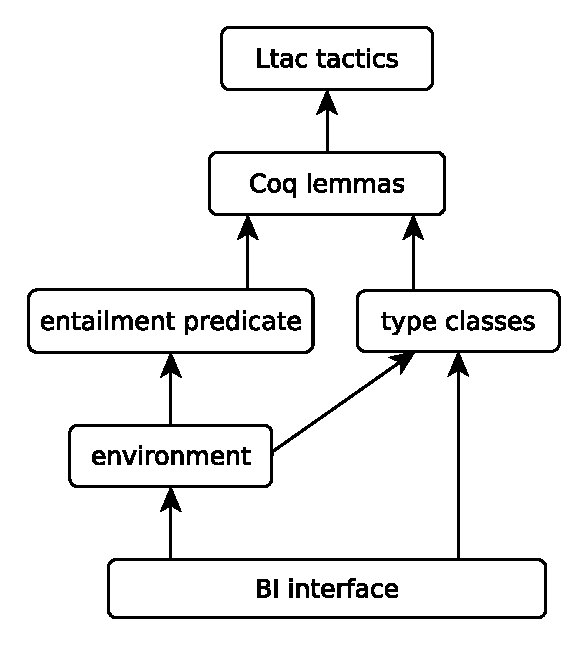
\includegraphics[width=0.5\linewidth]{ipm-diagram}
  \caption{Structure of the implementation of MoSeL}
  \label{fig:ipm-diagram}
\end{figure}

\begin{itemize}
\item The base layer of the implementation is a BI interface that the user instantiates with their logic and can use to profit from the existing infrastructure.
\item On top of the BI interface MoSeL defines environments and entailment predicates. These are used to make proofs of ``Coq tactics'' easier.
  Additionally, type classes allow for more general unification and proof search in an automated way.
\item ``Coq tactics'' themselves are verified transformations of the goal, the simplest instance being \coqe{tac_ex_falso}, which looks as follows:\\
  \coqe{Lemma tac_ex_falso Delta Q : envs_entails Delta False → envs_entails Delta Q.}, 
  where \coqe{envs_entails} is precisely the MoSeL entailment predicate.
  That is, a MoSeL proof state (without Coq context).
\item These transformations are then applied by Ltac1 (or Ltac2, in the reimplementation) programs, which can combine them, use specialized tactics for the subgoals they generate and handle errors.
  In this chapter we describe the Ltac1 implementation briefly and cover the translation in chapter~\ref{chap:ltac2-tactics-mosel}.
\end{itemize}

\subsubsection{BI interface}
\label{subsubsec:bi-interface}

There are five main components, starting with a base interface for BI logic, which we mentioned before and which \citet{krebbersMoSeLGeneralExtensible2018} call MoBI interfaces, for Modal BI.

We include it here, with some omissions:
\begin{coq}
Structure bi := Bi {
  bi_car :> Type;
  bi_dist : Dist bi_car;
  bi_emp : bi_car;
  bi_and : bi_car → bi_car → bi_car;
  bi_forall : forall A, (A → bi_car) → bi_car;
  bi_sep : bi_car → bi_car → bi_car;
  bi_wand : bi_car → bi_car → bi_car;
  bi_persistently : bi_car → bi_car;
  bi_pure : Prop → bi_car;
  bi_bi_mixin : BiMixin $\ldots$;
  $\ldots$
}.
\end{coq}

Where \coqe{BiMixin} is a field that describes axioms that connectives should satisfy, from associativity of separating conjunction to the elimination rule for persistent modality.
With some notation definitons this allows writing and proving BI propositions, only requiring an instance of \coqe{bi}.

\begin{minipage}{\linewidth}
\begin{coq}
Context {PROP : bi}.
Lemma persistently_mono P Q : (P |- Q) → <pers> P |- <pers> Q.
\end{coq}
\end{minipage}

Proving such a statement, however, at this point still requires applying axioms from \coqe{bi} by hand.

\subsubsection{Environments and the entailment predicate}
\label{subsubsec:environment-entailment-pred}

In order to define MoSeL entailment, we first define contexts.
In general, since most of the tactics only have to deal with one hypothesis from the context or don't even touch existing ones (like \coqe{iIntro}), \citet{krebbersMoSeLGeneralExtensible2018} use deep embedding to allow easier syntactical transformations.

Environments are defined as association lists with identifiers as keys and BI propositions as values.

\begin{coq}
Inductive ident :=
  | IAnon : positive -> ident
  | INamed :> string -> ident
Inductive env (A : Type) : Type :=
  | Enil : env A
  | Esnoc : env A -> ident -> A -> env A.
\end{coq}

As described above, however, MoSeL entailment predicate includes two contexts, spatial and intuitionistic, so we have to define another structure to include them both:

\begin{figure}[H]
\centering
\begin{coq}
Record envs (PROP : bi) := Envs {
  env_intuitionistic : env PROP;
  env_spatial : env PROP;
  env_counter : positive (** A counter to generate fresh hypothesis names *)
}.
\end{coq}
\caption{Definition of MoSeL environment in Coq}
\label{fig:coq_envs}
\end{figure}


Then we can define the entailment predicate, which includes not only both contexts, but also a proof that identifiers in each context are unique \coqe{$\ulcorner$ envs_wf $\Delta \urcorner$}.
\begin{coq}
  Definition envs_entails {PROP} ($\Delta$ : envs PROP) (Q : PROP):
  $\ulcorner$ envs_wf $\Delta \urcorner$ /\ $\intuit$ [$\wedge$] env_intuitionistic $\Delta$ * [*] env_spatial $\Delta$ |- Q
\end{coq}

Here \coqe{[*]} is an iterated separating conjunction, defined on lists as folds with the respective operation, the same way as it was defined in the theoretical presentation.

At this point we can already make some statements in both readable and easy to prove form, such as \coqe{tac_ex_falso}, which we mentioned before.

\begin{coq}
Lemma tac_ex_falso Delta Q : envs_entails Delta False → envs_entails Delta Q.
Proof. by rewrite envs_entails_eq -(False_elim Q). Qed.
\end{coq}

\subsubsection{Type classes}
\label{subsubsec:typeclasses}

Type classes serve multiple purposes in MoSeL development, and here we are going to describe only a couple of the simplest instances needed for \coqe{iAssumption}.
The primary idea is to automatize simple parts of proof search via logic programming.

The first example we are going to look at are \coqe{Affine} and \coqe{AffineEnv}.
The former is defined simply as
\begin{coq}
Class Affine {PROP : bi} (Q : PROP) := affine : Q |- emp.
\end{coq}

With instances covering both basic connectives
\begin{coq}
Global Instance emp_affine : Affine emp.
Global Instance and_affine_l P Q : Affine P → Affine (P /\ Q).
Global Instance and_affine_r P Q : Affine Q → Affine (P /\ Q).
Global Instance sep_affine P Q : Affine P → Affine Q → Affine (P * Q).
$\ldots$
\end{coq}

And modalities
\begin{coq}
Global Instance affinely_affine P : Affine (<affine> P).
$\ldots$
\end{coq}

For the environment to be affine we simply require all resources in the context to be affine and declare instances for both constructors.
\begin{coq}
Class AffineEnv (Γ : env PROP) := affine_env : Forall Affine Γ.
Global Instance affine_env_nil : AffineEnv Enil.
Global Instance affine_env_snoc Γ i P :
  Affine P → AffineEnv Γ → AffineEnv (Esnoc Γ i P).
\end{coq}

The next example is slightly more involved and concerns entailment of one proposition with another.
To be more precise, we want to define a type class which corresponds intuitively to ``\(P\) is almost the same as \(Q\) and P entails Q''.
\begin{coq}
Class FromAssumption {PROP : bi} (p : bool) (P Q : PROP) :=
  from_assumption : $\intuit$?p P |- Q.
\end{coq}
where \coqe{$\intuit$?p} is a technical connective which represents optional modality.

There are two subclasses of it, providing instances where either the first or the second proposition is treated as an input.
\begin{coq}
Class KnownLFromAssumption {PROP : bi} (p : bool) (P Q : PROP) :=
  knownl_from_assumption :> FromAssumption p P Q.
Class KnownRFromAssumption {PROP : bi} (p : bool) (P Q : PROP) :=
  knownr_from_assumption :> FromAssumption p P Q.
\end{coq}

The difference between their instances is that for \coqe{KnownLFromAssumption} we ``match'' input \(P\) with structural rules and Q is an output and vice-versa for \coqe{KnownRFromAssumption}.
This allows for more effective search, but for our purposes it is a mere technicality, so we will only consider \coqe{KnownRFromAssumption}.
The simplest instance we can declare is just an identity \coqe{P |- P}, which doesn't have to match either the left or the right input, so it uses \coqe{FromAssumption} directly.

\begin{coq}
Lemma from_assumption_exact {PROP : bi} p (P : PROP) : FromAssumption p P P.
\end{coq}

There are several more instances defined in MoSeL, which generalize it.
For example, given that we can prove \(\intuit P \vdash Q\), we can also prove  \(\intuit P \vdash \intuit Q\).
\begin{coq}
Global Instance from_assumption_intuitionistically_r P Q :
  FromAssumption true P Q → KnownRFromAssumption true P ($\intuit$ Q).
\end{coq}

\subsubsection{Coq tactics}
\label{sec:coq-tactics}

As mentioned above, Coq tactics are verified goal transformations, which can be as simple as rules for \coqe{exfalso}, but also more advanced, like the one for \coqe{assumption}.

The idea is that we have been provided with an identifier of the resource that is in the context and that we should check all side conditions: the resource is indeed there, it coincides with the goal and other resources can be safely discarded.

\begin{figure}[H]
\begin{coq}
Lemma tac_assumption Delta i p P Q :
  envs_lookup i Delta = Some (p,P) →
  FromAssumption p P Q →
  (let Delta' := envs_delete true i p Delta in
   if env_spatial_is_nil Delta' then TCTrue
   else TCOr (Absorbing Q) (AffineEnv (env_spatial Delta'))) →
  envs_entails Delta Q.
\end{coq}
\caption{\coqe{tac_assumption} definition}
\label{fig:tac-assumption}
\end{figure}

\coqe{envs_lookup} returns a boolean for the context in which it found identifier \coqe{i} and proposition \(P\) that was associated with the identifier.

The second assumption guarantees that \(P\) entails \(Q\) and the last one checks that we can discard the rest of the spatial resources in \(\Delta\).
If the spatial context is empty, there is nothing to discard, but otherwise either the whole environment must be affine, or the goal should be able to absorb them:
\(\Absorbing P \defeq \forall Q, P * Q \vdash P\).

No other subgoals are generated, since this is a leaf of a derivation.

\subsubsection{Ltac tactics}
\label{sec:ltac1-tactics}

The final piece of the puzzle is the Ltac layer.
While Coq lemmas, such as in figure~\ref{fig:tac-assumption}, are essentially functions from one proof state to another, applying them by hand to do proofs is still pretty far from proper Coq tactics.
To this end, MoSeL uses Ltac functions that apply necessary lemmas, perform bookkeeping and handle subgoals.
This introduces a balance between what should go into a Coq statement and an Ltac1/Ltac2 function, since we want to provide input for Coq lemmas automatically.

For example, in order to apply \coqe{tac_assumption} for a specific resource \coqe{j : P}, in the spatial context, we would have to write the following:

\begin{figure}[H]
\begin{coq}
Tactic Notation "iExactSpatial" constr(H) :=
  eapply (tac_assumption _ j false P);
    [pm_reflexivity (* for the lookup *)
    |iSolveTC (* perform type class search for FromAssumption*)
    |pm_reduce; (* evaluate env_delete and if-branch *)
     iSolveTC]
\end{coq}
\caption{Implementation of iExact for spatial context}
\label{fig:ltac1-iassumption}
\end{figure}

We apply the \coqe{tac_assumption} defined earlier (figure~\ref{fig:tac-assumption}) and discharge the goals with specialized tactics.
The first subgoal \coqe{envs_lookup i Delta = Some (p,P)} is computational, so \coqe{pm_reflexivity} performs evaluation and uses \coqe{reflexivity} tactic.
The other two concern type classes, so we use a wrapper around \coqe{typeclasses eauto} to solve them.
\coqe{iExactSpatial} is not a real tactic, since it's too specialized, but it is correct.

\coqe{iAssumption}, on the other hand, is a bit more complicated and we will go through it in the next chapter.

%%% Local Variables:
%%% mode: latex
%%% TeX-master: "thesis"
%%% TeX-parse-self: t
%%% TeX-auto-save: t
%%% reftex-cite-format: natbib
%%% reftex-default-bibliography: ("/home/buzzer/my-dir/ed/uni/saar/prjcts/iris/npm/tex/TacticsProofs.bib")
%%% End: